\documentclass[10pt,a4paper]{article}
\usepackage{xcolor}
\definecolor{ocre}{RGB}{243,102,25}
\usepackage[utf8]{inputenc}
\usepackage{amsmath}
\usepackage{amsfonts}
\usepackage{amssymb}
\usepackage{graphicx}
\usepackage{algpseudocode}
\usepackage{algorithm}

\title{Rejection Sampling}


\begin{document}
\maketitle 

Rejection sampling is a sampling algorithm to sample data from a complex multivariate distribution using a proxy distribution.
\\

Let's set up the scenario. Assume our target distribution $p(x)$ is easy to sample from but only up to a normalizing constant $Z$. So,

\begin{align*}
p(x) = \frac{\tilde{p}(x)}{Z}
\end{align*}

\vspace{0.3cm}
\noindent where $\tilde{p}(z)$ is easy to sample from. Let $q(z)$ be any distribution that is easy to sample from. $q(z)$ is called the \textit{proposal distribution}. Define $kq(z)$ such that it `blankets' $\tilde{p}(z)$ (in other words, $kq(z) \geq \tilde{p}(z)$). See Figure 1 below.

\begin{figure}[!h]
\centering
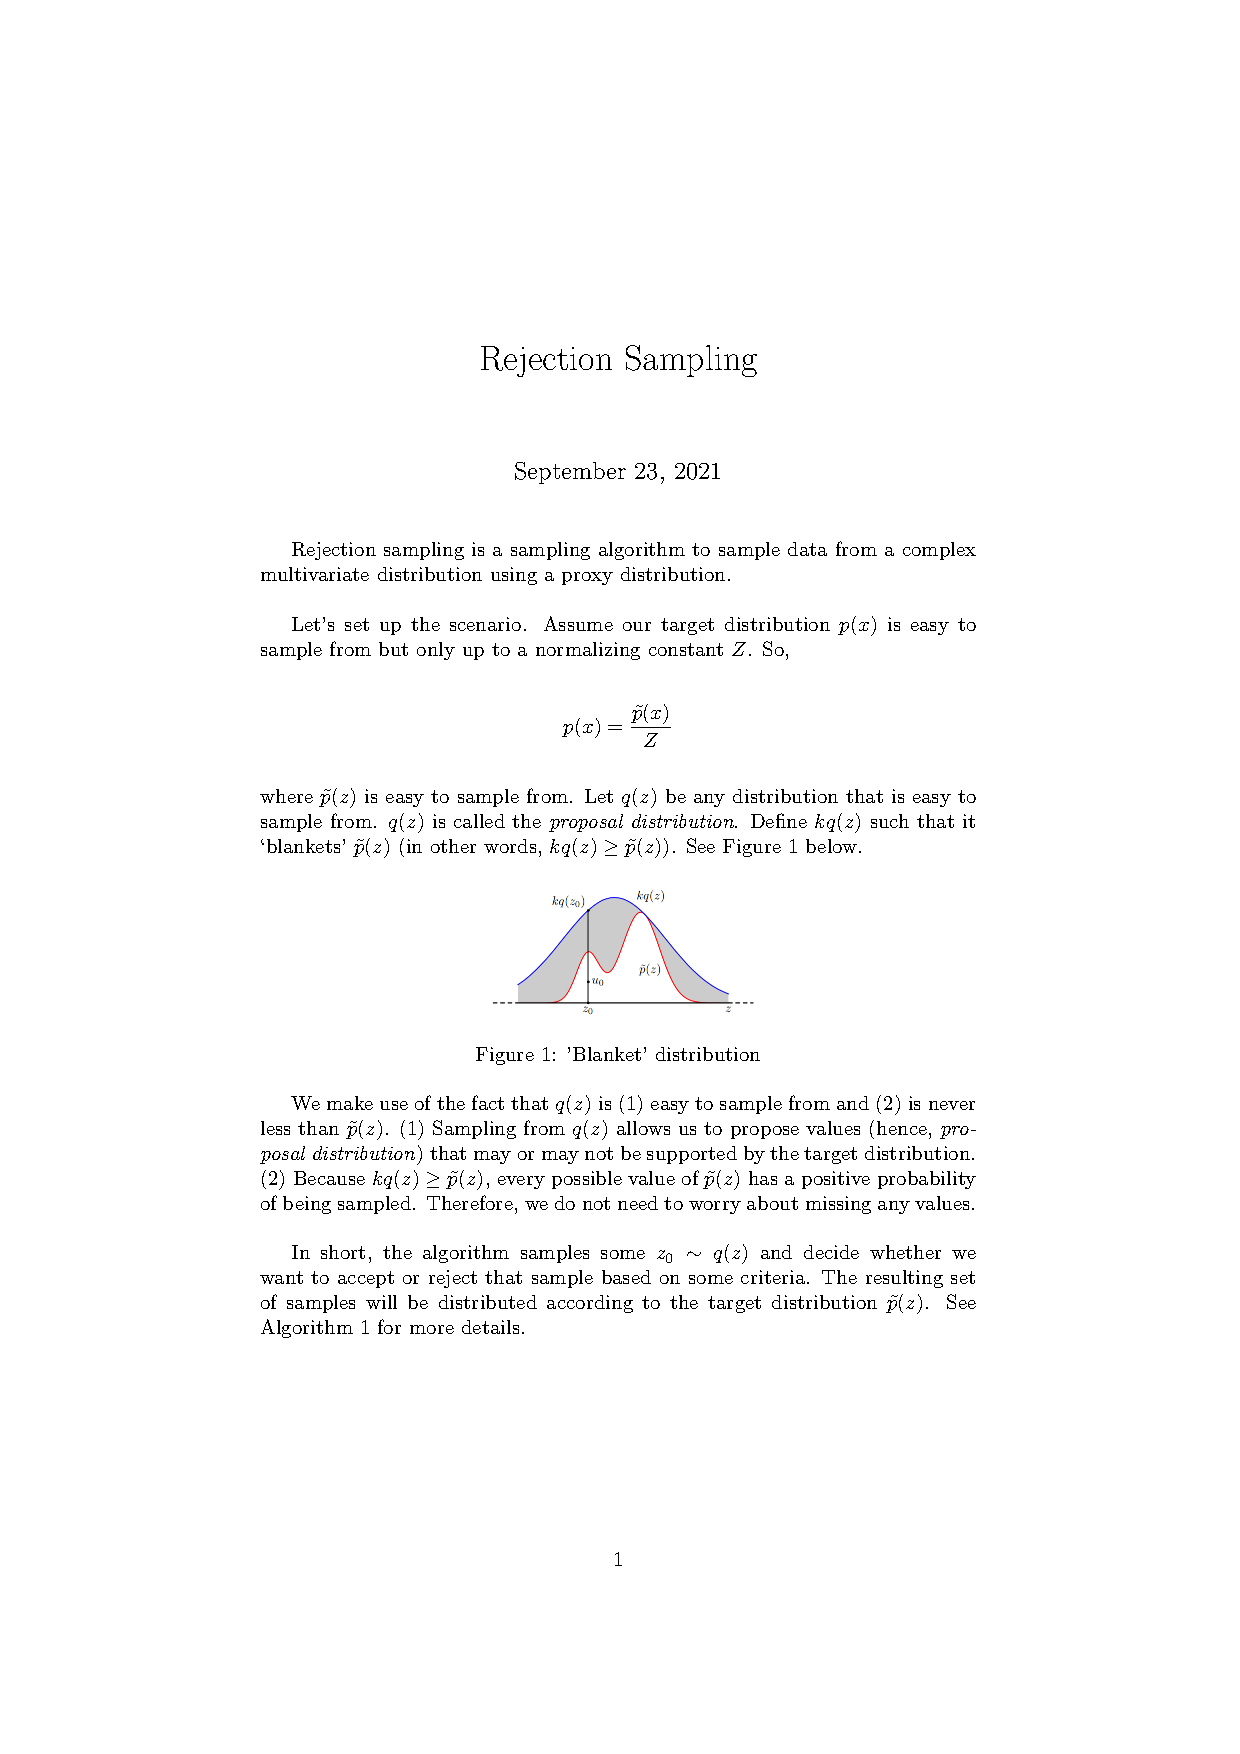
\includegraphics[scale=0.4]{figures/rejection_sampling.png}
\caption{'Blanket' distribution}
\end{figure}


We make use of the fact that $q(z)$ is (1) easy to sample from and (2) is never less than $\tilde{p}(z)$. (1) Sampling from $q(z)$ allows us to propose values (hence, \textit{proposal distribution}) that may or may not be supported by the target distribution. (2) Because $kq(z) \geq \tilde{p}(z)$, every possible value of $\tilde{p}(z)$ has a positive probability of being sampled. Therefore, we do not need to worry about missing any values.
\\

In short, the algorithm samples some $z_0 \sim q(z)$ and decide whether we want to accept or reject that sample based on some criteria. The resulting set of samples will be distributed according to the target distribution $\tilde{p}(z)$. See Algorithm 1 for more details.

\vspace{0.5cm}

\begin{algorithm}
\caption{Rejection Sampling}
\begin{algorithmic}
\State $z_0 \sim q(z)$
\State $u \sim U(0, kq(z_0))$
\If{$u \leq \tilde{p}(z_0)$}
	\State Accept
\Else
	\State Reject
\EndIf
\end{algorithmic}
\end{algorithm}

\pagebreak

\section{Notes}
\begin{itemize}
\item Complex target function f(x)
\item Proposal function g(x)
\item Scale g(x) with some constant c to ‘blanket’ the target function -- cg(x)
\item Sample some $x_0 \sim g(x)$
\item $x_0$ will be a valid input to our distribution if f(x) and g(x) have the same range
\item Compute $cg(x_0)$ and $f(x_0)$
\item Sample $u \sim U(0, cg(x))$
\item Our acceptance criterion is $u \leq f(x)$
\item Alternate formulation (more common):
\item Acceptance criterion: $u \leq f(x)/cg(x)$
\item Sample $u \sim U(0, 1)$
\end{itemize}

\end{document}